% здесь также можно добавить обложку
\begin{titlepage}
    \vspace*{\fill}
    \begin{center}
      
\includegraphics[width=\textwidth]{dead-pineapple.pdf}
    \end{center}
    \vspace*{\fill}
    \begin{center}
        \author\\\the\year
    \end{center}
\end{titlepage}

\section*{Вместо предисловия}
\vspace*{\fill}
От создателей без\emph{цели}ра \href{https://antoniii.github.io/}{100 идей для стартапа}.
Они вернулись чтобы творить... но лень!\\

\emph{\Huge{ZZZ}\LARGE{ZZZ}\Large{ZZZ}\large{ZZZ}ZZZ\small{ZZZ}\footnotesize{ZZZ}\scriptsize{ZZZ}\tiny{ZZZ}\tiny{zzz}}

\vfill

\begin{center}
    Сотрудники \author: % издательства свободных художников-исследователей слова. Сокр. СИСХИС
    \begin{itemize}
        \item Алекс ---  автор-исследователь и {\TeX}нический редактор
        \item Антонио --- автор-критик и \rotatebox[origin=c]{180}{\tiny промышленный шпион}
        \item Вальдемар --- автор-стилист и \( \pi\iota\zeta o \nu \) компании
        \item Илиа --- автор-эстет и {\fontfamily{antt}\selectfont\scshape художественный} редактор
    \end{itemize}
    
\begin{figure}[ht!]
    \centering
    
\includegraphics[width=\textwidth]{we}
\end{figure}

    \vfill
    Благодарности:
    \begin{itemize}
        \item Серхио за роль пассивно-заочного критика
        \item Николаю Васильевичу за его великую повесть <<Записки сумасшедшего>>
    \end{itemize}
\end{center}

\vfill

\newpage

\begin{epigraph}
Однажды к Эйнштейну пришёл журналист.\\
--- Куда вы записываете свои мысли?~--- спросил он.~--- У вас есть для этого блокнот или записная книжка?\\

Эйнштейн ответил:\\
--- Милый мой! Настоящие мысли приходят в голову так редко, что их нетрудно и запомнить.
\end{epigraph}

\begin{figure}[ht!]
    \centering
    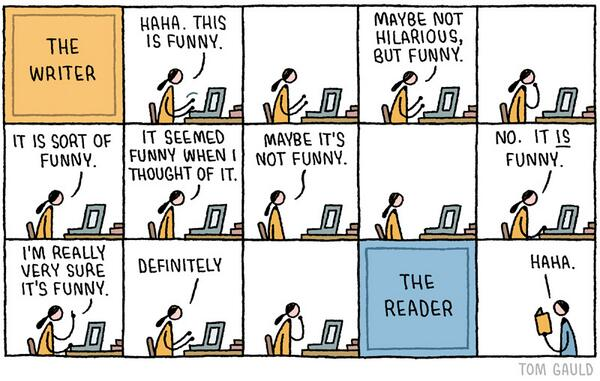
\includegraphics[width=\textwidth]{ideas}
\end{figure}

\newpage

\section*{А что ты сделал для hip-hop'a в свои годы?}\label{section:one}
\begin{epigraph}
        Мы обожаем книги мёртвых наркоманов\\
        {\normalfont Рөстәм Баян улы Булатов, 2 июня 2015}
\end{epigraph}
Зачем всё это? Попытка создать новый жанр в литературном творчестве.
А если без пафоса, то это пародия, попытка стёба потуг оных. Ибо ныне излишне много развелось всяких псевдописателей (не поминая уже армию разномастных блоггеров).

\begin{figure}[ht!]
    \centering
    
\includegraphics[width=\textwidth]{hip-zen}
\end{figure}
